\documentclass{beamer}
\usetheme{Copenhagen}
\usecolortheme{spruce}
\usepackage{ctex}
\usepackage{eulervm}
\usefonttheme{professionalfonts}
\renewcommand{\rmdefault}{pplx}
\usepackage{listings}
\usepackage{url}

\title{小学数学思维潜力课 / 序言}
\author{张昆玮}

\begin{document}
\begin{frame}
\maketitle
\end{frame}

\begin{frame}{初衷:解决家长的困惑}
\begin{exampleblock}{家长的困惑}
为什么自家孩子在小学看上去都是双百分,\\
\qquad 上了中学之后却因为没有潜力,逐渐退步?\\
\bigbreak
为什么自家孩子找不到学习的动力,\\
\qquad 或者学习得很辛苦却没有回报?\\
\end{exampleblock}
\bigbreak
现在的小学课堂,只注重知识掌握,缺乏方法培养,\\
\qquad 没能挖掘出学生的潜力!\\
\bigbreak
梦圆教育特邀清华“姚班”毕业生张昆玮回到榆次,\\
\qquad 开设小学数学思维潜力课程!\\
\end{frame}

\begin{frame}{教师简介 -- 张昆玮}
\begin{center}
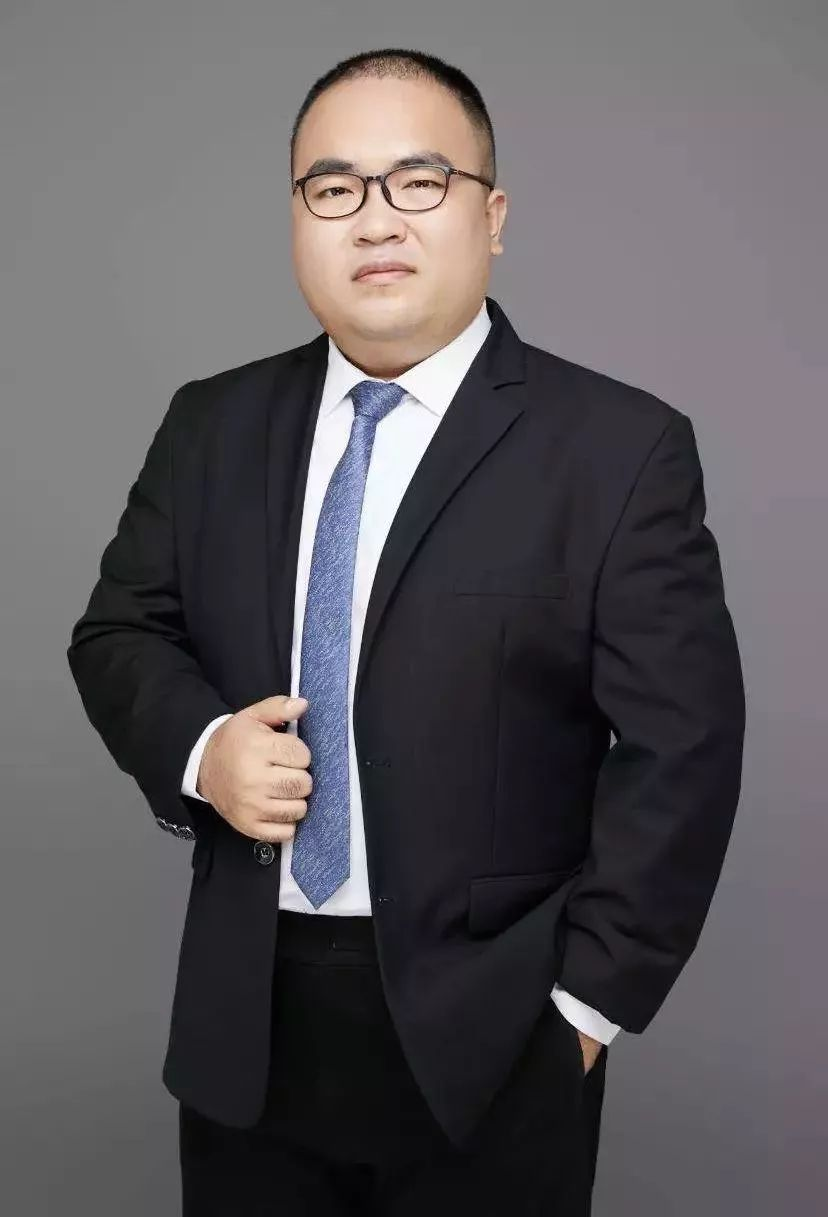
\includegraphics[width=.2\textwidth]{image/照片.jpg}
\end{center}
就读\textbf{太行小学},小学时就在数学方面展现出非凡潜力;\\
进入\textbf{榆次五中},两次获得希望杯金牌,联赛山西省第一名。\\
高中\textbf{山西省实验中学},获高中数学、物理联赛山西省一等奖,\\
计算机竞赛全国金牌,保送\textbf{清华大学}后进入姚班
\footnote{姚班是清华大学培养计算机学科拔尖创新性人才的摇篮,每年在全国仅招 $30 \sim 40$ 人,是名副其实的尖子班,精英班。},\\
清华读完硕士,先后在\textbf{摩根大通、谷歌}等著名企业工作。
\end{frame}

\begin{frame}{培养学生潜力的重要性}
\begin{itemize}
\item 身为三晋学子,张昆玮感到:\\
山西的教育资源与北京、上海等经济发达地区的差距\\
在最近几年并没有缩小,而是拉大了。
\item 在中国教育资源最丰富、最强大、最顶尖的北京海淀区,\\
父母们拼着十几万一平的学区房,\\
给孩子报着几百甚至上千块一节的奥数课,\\
并且在后方这样尽心尽力地跟着。
\item 而在山西,很多人还蒙在鼓里,觉得能学好知识就够了,\\
不懂得培养孩子的潜力。
\end{itemize}
\bigbreak
是这些北京的父母傻吗?不是。仅仅就这一个海淀区,\\
中国包括清华、北大、人大等 30 多所名校扎堆在这里,\\
而最好的小学、中学、高中,也集中在这里。\\
父母们太知道让孩子赢在起跑线上的重要性了。\\
没有生来如此的优秀,只有百炼成钢的坚持。
\end{frame}

\begin{frame}{学习计划}
开课年级:小学四五六年级,分班上课。\\
开课时间:暑假、秋季学期、春季学期各 $15$ 节课。\\
\bigbreak
暑假课表:\\
09:00 -- 11:00 新四年级\\
14:00 -- 16:00 新五年级\\
16:00 -- 18:00 新六年级\\
\end{frame}

\begin{frame}{教材和教学大纲}
采用教材:《奥数精讲与测试》二至六年级\\
\bigbreak
四年级暑假:原书二年级上\\
四年级秋季:原书二年级下、三年级上\\
四年级春季:原书三年级下\\
五年级暑假:原书四年级上\\
五年级秋季:原书四年级下\\
五年级春季:原书五年级上\\
六年级暑假:原书五年级下\\
六年级秋季:原书六年级上\\
六年级春季:原书六年级下\\
\end{frame}

\begin{frame}{问答环节}
请学生和家长就课程内容踊跃提问。
\end{frame}
\end{document}
